%==========================================================
\subsection{Unbinding Particles}\label{chap:unbinding}
%==========================================================


A further requirement for substructure finding is the removal of energetically unbound particles, i.e. assigning a particle originally located within a substructure to the parent structure based on an energy criterion. 
This applies recursively to any level of substructure within substructure. 
Such a hierarchical clustering of matter is expected due to self gravity.
It is customary to treat all particles assigned to a halo as bound to it, even though from a strict energetic perspective they are not, thus particle unbinding may not be necessary for haloes, but it is vital for subhaloes. 
Subhaloes are by definition located within a host halo and are therefore expected to be contaminated by the host's particles.
Considering that substructure often contains far fewer particles than its host, blindly assigning particles to it without an unbinding procedure can influence its physical properties significantly. 


Various techniques to identify unbound particles within the found structures are used as well.
Because removing particles from a structure changes said structures properties, often iterative approaches are used.
\texttt{AHF} \parencite{AHF}, \texttt{ASOHF} \parencite{ASOHF} and \texttt{SUBFIND} \parencite{subfind} for example remove all unbound particles from a halo, recompute the potential and repeat the procedure until no more particles are removed.
Unbound particles are then passed from subhaloes on to host haloes (or host subhaloes) for examination.
\texttt{SKID} \parencite{skid} however only removes the particle with the highest energy per iteration.










By considering an isolated clump in a time-independent scenario, where energy is conserved, a particle $i$ is considered to be bound if its total energy $E_i$
%
\begin{align}
	E_i = \frac{1}{2} m_i \cdot v^2_i + m_i \phi (\mathbf{r}_i)\label{eq:E}
\end{align}
%
is negative:
\begin{align}
	& E_i < 0 &\Leftrightarrow \text{ particle is bound } &\\
	\Rightarrow \quad & 	v_i < \sqrt{- 2 \cdot \phi(\mathbf{r}_i)} &\Leftrightarrow \text{ particle is bound }\label{eq:boundv}
\end{align}

where $\mathbf{r}_i$ is the particle's position, $v_i = ||\mathbf{v}_i||$ is the magnitude of the particle's velocity, both given in the centre of mass frame of the clump, and $m_i$ is the mass of every particle $i$.
Approximating the clump as a spherically symmetric object, the Poisson equation (eq. \eqref{eq:poisson}) reduces from a three-dimensional problem to a one-dimensional one, as the potential $\phi(\mathbf{r})$ will only depend on the absolute distance from the origin, $r_i \equiv ||\mathbf{r_i}||$, not any angular direction.
For this case, the Poisson equation for the gravitational potential $\phi$ can be solved analytically under the assumption that $\phi(r\rightarrow\infty) \rightarrow 0$:
%
\begin{align}
	\phi (r_i) &=  - G \int\limits_{r_i}^{r_{max}} \frac{M(<\tilde{r})}{\tilde{r}^2} \mathrm{d}\tilde{r}
	- G  \frac{M_{tot}}{r_{max}}
	\label{eq:sol_phi}\\
%
	 M(<r) & \equiv \int\limits_0^r 4 \pi \rho(\tilde{r})\tilde{r}^2 \mathrm{d}\tilde{r}
\end{align}
%
Where $M(<r)$ is the mass enclosed by a sphere of radius $r$ such that the clump's total mass is enclosed by the radius $r_{max}$: $M_{tot} = M(<r_{max})$.




One problem with this condition is that it assumes that clumps will be isolated, which by construction of the clump finder \phew\ subhaloes will never be.
The issues that arise from this fact can be understood by considering the boundaries of a particle's trajectory.
These boundaries in a given potential $\phi$ can be estimated using the conservation of energy:
%
\begin{align}
	E/m_p = \frac{1}{2} v^2 + \phi = const.
\end{align}
%
A gravitational potential is qualitatively shown in figure \ref{fig:orbits} as well as a particle $\alpha$ with $\frac{1}{2}v^2 < - \phi$.
The total energy per particle mass $E/m_p$ of the particle on the graph is then exactly the difference between the negative potential and the kinetic energy on the $y$-axis.
In order to conserve energy, the curve of possible kinetic energies (dotted line in figure \ref{fig:orbits}) that the particle may take on will always have the same distance $E/m_p$ from the negative potential curve.
Because $v^2\geq 0$, the spatial boundaries of a particle's trajectory can be found by following the curve of possible kinetic energies of the particle to the points where $v^2 = 0$.

\begin{figure}[h!]
	\centering
	\minipage[t]{0.44\textwidth}
	%\centering
	\fbox{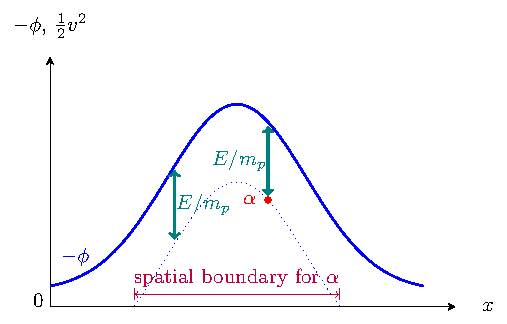
\includegraphics[height=4.45cm, keepaspectratio]{images/tikz/boundaries.pdf}}%
	\caption{A qualitative plot of a potential $\ -\phi$ and a particle $\alpha$. 
		The boundaries of the particle's trajectory can be found using energy conservation $E/m_p = \frac{1}{2}v^2 + \phi = const$ by following the curve of the particle's kinetic energies (dotted line) to the points where $v^2=0$.	
	}%
	\label{fig:orbits}
	\endminipage%\hspace{.1cm}
	\hspace*{\fill}
	%
	\minipage[t]{0.54\textwidth}
	%\centering
	\fbox{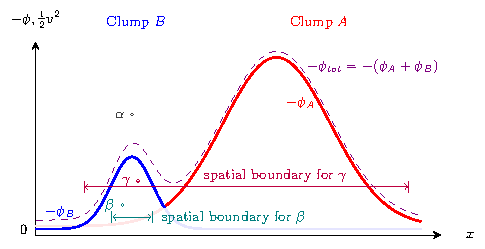
\includegraphics[height=4.45cm, keepaspectratio]{images/tikz/potentials.pdf}}%
	\caption{Qualitative potential of a halo containing two clumps $A$ and $B$. Three particles assigned to $B$ are shown: $\alpha$ is not bound to $B$, $\beta$ is bound, $\gamma$ satisfies the energy condition to be bound, but can wander off into clump $A$ and shouldn't be considered as such.
	}%
	\label{fig:potentials}
	\endminipage\hspace*{\fill} 
\end{figure}
%
This fact changes the situation significantly for the interpretation of what particles should be considered bound as follows.
Consider now an isolated halo that consists of two clumps, $A$ and $B$, where $B$ is a smaller clump nested within clump $A$.
Their potentials are qualitatively depicted in figure \ref{fig:potentials}. 
Three particles assigned to $B$ with different kinetic energies are marked, representing three different cases:
%
\begin{itemize}
	\item Particle $\alpha$ has a kinetic energy higher than the potential, it is clearly not bound to the clump $B$.
	\item Particle $\beta$ has a kinetic energy lower than the potential at that distance from the centre of mass, so it will remain bound on an elliptic trajectory around the centre of mass.
	\item Particle $\gamma$ is considered energetically bound to the clump just like $\beta$, i.e. it satisfies condition \eqref{eq:boundv}, but it won't necessarily remain on an elliptic trajectory around clump $B$'s centre of mass: Because of clump $A$'s neighbouring potential, the particle can leave the boundaries of clump $B$ and wander off deep into clump $A$.
\end{itemize}
%

These considerations show that due to the fact that subhaloes will always have neighbouring structure by definition, there will be particles like $\gamma$ that can wander off into neighbouring clumps even though they satisfy condition \eqref{eq:boundv}.
It is obvious that particles like $\gamma$ shouldn't be considered as bound and that therefore the condition for a particle to be bound needs to be modified appropriately.
Since the reason $\gamma$ can wander off is because its boundary extends past the interface that connects the two clumps, the condition for a particle to be bound must be that its trajectory must never reach that interface.
Defining $\phi_S$ to be the potential of clump $B$ at the interface to the neighbouring structure that is closest to $B$'s centre of mass, the condition for a particle to be bound \emph{exclusively} to a particular clump can be written as
%
\begin{align}
	E/m_p = \frac{1}{2}v^2 + \phi -  \phi_S < 0
\end{align}
%
or equivalently:
%
\begin{align}
	v < \sqrt{ - 2(\phi - \phi_S) } \label{eq:boundv_corr}
\end{align}


According to the argumentation above and figures \ref{fig:orbits} and \ref{fig:potentials}, it is to be expected that demanding particles to be exclusively bound will find more unbound particles than not doing so, where particles close to the centre of mass should be more likely to be exclusively bound than the particles closer to the edge of the subhalo.



